% !TEX root = ./Basilisk-spacecraftPointing-20190116.tex

\section{Model Description}

\subsection{Module Goal}\label{subsec:goal}

This module is intended for controlled formation flying applications where it is necessary to set up at least a chief spacecraft and a deputy spacecraft. The goal of this module is to align a vector defined by the user in the deputy body frame ($^{\cal B}{\bm a}$) with a vector that points from the deputy to the chief spacecraft ($^{\cal N}{\bm \rho}$). Both vectors are displayed in Fig.~\ref{fig:rel_point}. The $^{\cal B}{\bm a}$ vector defined by the user can, for instance, be the location of an antenna or a camera within the body frame. Besides the $^{\cal B}{\bm a}$ vector, the module uses the location of the chief and deputy spacecraft in the inertial frame as an input. The outputs of this module consist of the orientation of a reference frame that is built around the $^{\cal N}{\bm \rho}$ vector, the angular velocity of the reference frame, and the angular acceleration (all with respect to the inertial frame). Together with the attitude of the deputy spacecraft body frame, the outputs of this module can be fed into the attitude tracking error module. This module consequently calculates the error between the reference frame built around the $^{\cal N}{\bm \rho}$ vector and the spacecraft body frame to make sure that the body frame eventually aligns with this reference frame. 

\subsection{Equations}

As discussed in Sec.~\ref{subsec:goal} the inputs of this module are the position of the chief and the deputy spacecraft with respect to the inertial frame ($^{\cal N}{\bm r}_{\textrm{chief}}$ and $^{\cal N}{\bm r}_{\textrm{deputy}}$ respectively). In order to find the unit vector that points from the deputy to the chief Eq.~\eqref{eq:rho_norm} can be used.

\begin{equation}
    ^{\cal N}\hat{{\bm \rho}} = \frac{^{\cal N}{\bm r}_{\textrm{chief}} - ^{\cal N}{\bm r}_{\textrm{deputy}}}{||^{\cal N}{\bm r}_{\textrm{chief}} - ^{\cal N}{\bm r}_{\textrm{deputy}}||}
    \label{eq:rho_norm}
\end{equation}

\begin{figure}[htb]
	\centerline{
	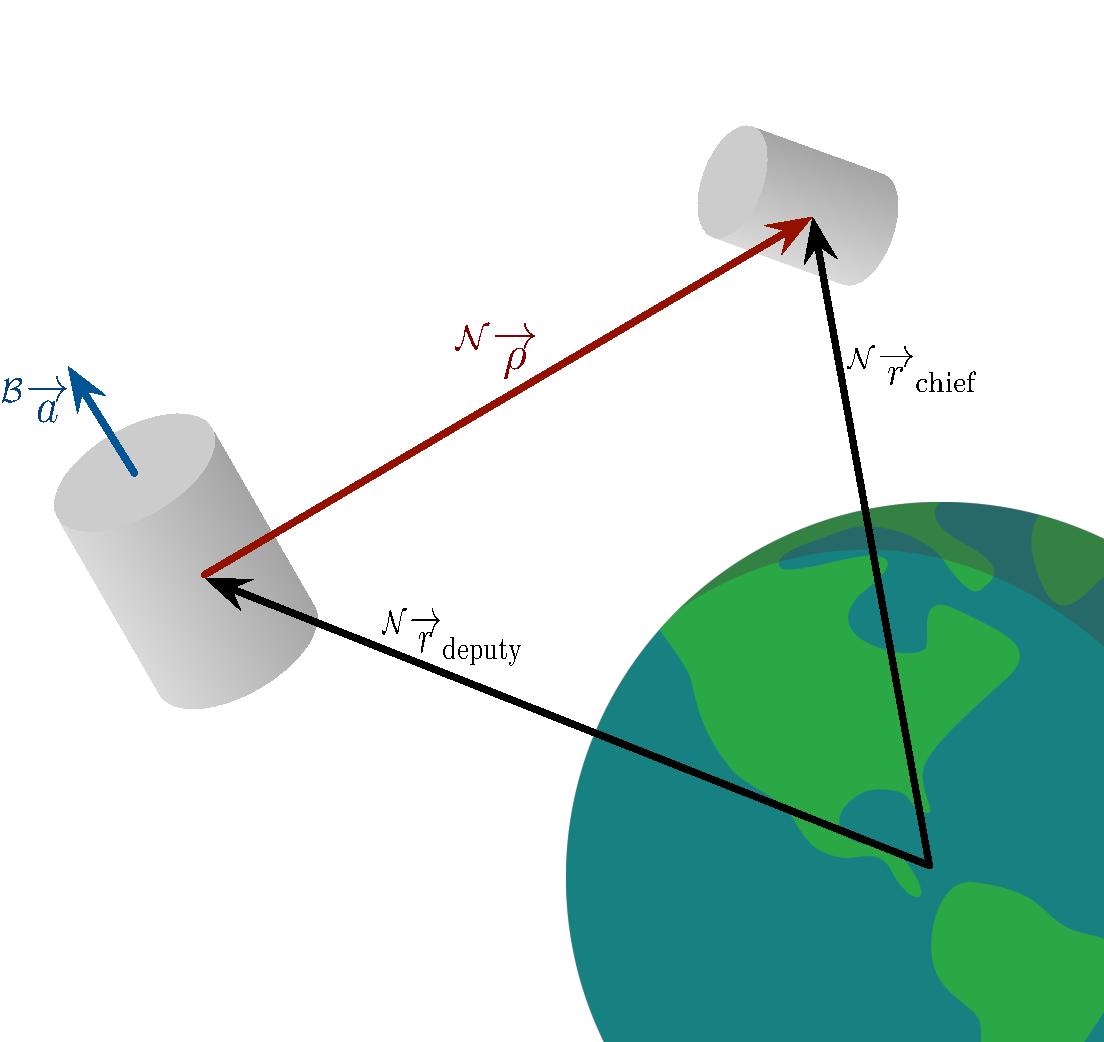
\includegraphics[scale=0.52]{Figures/relativePointing.pdf}
	}
	\caption{Vector illustrations}
	\label{fig:rel_point}
\end{figure}

Consequently, a coordinate system is built around the $^{\cal N}\hat{{\bm \rho}}$ vector as can be seen in Eq.~\eqref{eq:R-coordinates}. In this equation, ${^{\cal N}\hat{{\bm x}}}$, ${^{\cal N}\hat{{\bm y}}}$, and ${^{\cal N}\hat{{\bm z}}}$ are the normalized x-, y-, and z-components of the $\cal R$ frame written in $\cal N$ frame components. Furthermore, ${\hat{\bm z}}$ represents the z-component in the $\cal N$ frame ($[0,0,1]^{T}$). The entries in the direction cosine matrix (dcm) can be observed in Eq.~\eqref{eq:dcm_RN}. 

\begin{equation}
    \begin{split}
    {^{\cal N}\hat{{\bm x}}} &= {^{\cal N}\hat{{\bm \rho}}} \\
    {^{\cal N}\hat{{\bm y}}} &= {\hat{\bm z}} \times {^{\cal N}\hat{{\bm \rho}}} \\
    {^{\cal N}\hat{{\bm z}}} &= {^{\cal N}\hat{{\bm x}}} \times {^{\cal N}\hat{{\bm y}}}
    \end{split}
    \label{eq:R-coordinates}
\end{equation}

\begin{equation}
    [RN] = \begin{bmatrix}
            {^{\cal N}\hat{{\bm x}}}^{T}\\ 
            {^{\cal N}\hat{{\bm y}}}^{T}\\ 
            {^{\cal N}\hat{{\bm z}}}^{T}
            \end{bmatrix}
            \label{eq:dcm_RN}
\end{equation}

Using the "C2MRP" function in C this dcm is converted to the Modified Rodrigues Parameter (MRP) vector ${\bm \sigma}_{RN}$.\\
\\
Consequently, it is possible to calculate the angular velocity of the $\cal R$ frame with respect to the $\cal N$ frame in $\cal N$ frame components. In order to find the angular velocity ${\bm \sigma}_{RN}$ at time $\textrm{t-1}$ is subtracted from ${\bm \sigma}_{RN}$ at time $\textrm{t}$  and divided by the timestep ($\Delta \textrm{t}$) as can be seen in Eq.~\eqref{eq:sigma_dot}.

\begin{equation}
    \dot{\bm \sigma}_{RN} = \frac{{\bm \sigma}_{RN}(\textrm{t}) - {\bm \sigma}_{RN}(\textrm{t-1})}{\Delta \textrm{t}}
    \label{eq:sigma_dot}
\end{equation}

After that, the angular velocity of the $\cal R$ frame with respect to the $\cal N$ frame in $\cal R$ frame components can be computed using Eq.~\eqref{eq:omega_eq} (equation 3.164 in Analytical Mechanics of Space Systems \cite{Schaub}). The sigma components used in this equation are the average sigma between sigma at $\textrm{t-1}$ and sigma at $\textrm{t}$. This is done due to the fact that using the sigma components at solely time $\textrm{t}$ results in incorrect values for omega. In case the chief would orbit the deputy circularly with a known rate it turns out that the results from the numerical method fluctuate around the true angular velocity. Taking the average of sigma results in an angular velocity that is in coherence with values calculated analytically and is constant up to $10^{-9}$. Using a dcm $^{\cal N}{\bm \omega}_{RN}$ is calculated from $^{\cal R}{\bm \omega}_{RN}$. Finally, the angular acceleration ($^{\cal N}\dot{\bm \omega}_{RN}$) can be calculated using Eq.~\eqref{eq:domega}.

\begin{equation}
    ^{\cal R}{\bm \omega}_{RN} = \frac{4}{(1 + \sigma^{2})^{2}}[(1-\sigma^{2})[I_{3 \times 3}] - 2[\widetilde{\bm \sigma}] + 2{\bm \sigma}{\bm \sigma}^{T}]\dot{\bm \sigma}_{RN}
    \label{eq:omega_eq}
\end{equation}

\begin{equation}
    ^{\cal N}\dot{\bm \omega}_{RN} = \frac{^{\cal N}{\bm \omega}_{RN}(\textrm{t}) - ^{\cal N}{\bm \omega}_{RN}(\textrm{t-1})}{\Delta \textrm{t}}
    \label{eq:domega}
\end{equation}

As stated in Sec.~\ref{subsec:goal}, the attitude tracking error module calculates the error of the deputy spacecraft's attitude with respect to the attitude of the reference frame (the ${\cal R}$ frame). For this reason, using ${\bm \sigma}_{RN}$ would result in an alignment of the x-axis of the deputy spacecraft's body frame with the $^{\cal N}\hat{{\bm \rho}}$ vector instead of an alignment of the vector specified by the user ($^{\cal B}{\bm a}$) with the $^{\cal N}\hat{{\bm \rho}}$ vector. So instead of using the ${\cal R}$ frame as one of the outputs of this module, it is necessary to create a different coordinate frame. The name of this frame is the ${\cal R}_{1}$ frame and in case the ${\cal B}$ frame aligns with the ${\cal R}_{1}$ frame, $^{\cal B}{\bm a}$ has to align with $^{\cal N}{\bm \rho}$. For this reason, an ${\cal A}$ frame is built around the $^{\cal B}{\bm a}$ vector. The creation of this coordinate frame can be found in the Reset function in the code. The vector components of this coordinate system can be seen in Eq.~\eqref{eq:A-coordinates}. In this equation, ${\hat{\bm z}}$ represents the z-component of the body frame.

\begin{equation}
    \begin{split}
    {^{\cal B}\hat{{\bm x}}} &= {^{\cal B}\hat{{\bm a}}} \\
    {^{\cal B}\hat{{\bm y}}} &= {\hat{\bm z}} \times {^{\cal B}\hat{{\bm a}}} \\
    {^{\cal B}\hat{{\bm z}}} &= {^{\cal B}\hat{{\bm x}}} \times {^{\cal B}\hat{{\bm y}}}
    \end{split}
    \label{eq:A-coordinates}
\end{equation}

The dcm that consequently maps the ${\cal B}$ frame to the ${\cal A}$ frame can be found in Eq.~\eqref{eq:dcm_AB}.

\begin{equation}
    [AB] = \begin{bmatrix}
            {^{\cal B}\hat{{\bm x}}}^{T}\\ 
            {^{\cal B}\hat{{\bm y}}}^{T}\\ 
            {^{\cal B}\hat{{\bm z}}}^{T}
            \end{bmatrix}
            \label{eq:dcm_AB}
\end{equation}

This dcm is transformed in ${\bm \sigma}_{AB}$ using the "C2MRP" function in C. \\
\\
In order to make sure that the ${\cal A}$ frame aligns with the ${\cal R}$ frame (meaning that $^{\cal B}{\bm a}$ aligns with $^{\cal N}\hat{{\bm \rho}}$), the following computations are performed and illustrated using a 2D example. Looking at Fig.~\ref{fig:coordinate_systems} the orientation of the ${\cal N}$ frame can be observed. Besides that, it is possible to see a ${\cal B}$ frame and an ${\cal A}$ frame relative to this ${\cal B}$ frame. Furthermore, Fig.~\ref{fig:coordinate_systems} shows the orientation of the ${\cal R}$ frame and the ${\cal R}_{1}$ frame. Up until this point ${\bm \sigma}_{RN}$ and ${\bm \sigma}_{AB}$ are calculated. The goal is to align the ${\cal A}$ frame with the ${\cal R}$ frame. This is the same as aligning the ${\cal B}$ frame with the ${\cal R}_{1}$ frame (noting that ${\bm \sigma}_{AB}$ = ${\bm \sigma}_{RR_{1}}$). For this reason, the reference MRP that will be used as an output is ${\bm \sigma}_{R_{1}N}$ and can be calculated using Eq.~\eqref{eq:sigma_R1N} (because ${\bm \sigma}_{BA} = - {\bm \sigma}_{AB}$).

\begin{equation}
    {\bm \sigma}_{R_{1}N} = {\bm \sigma}_{RN} + {\bm \sigma}_{BA}
    \label{eq:sigma_R1N}
\end{equation}

The angular velocity and angular acceleration stay the same because both the angular velocity and the angular acceleration of the ${\cal A}$ frame with respect to the ${\cal B}$ frame are constant.

\begin{figure}[htb]
	\centerline{
	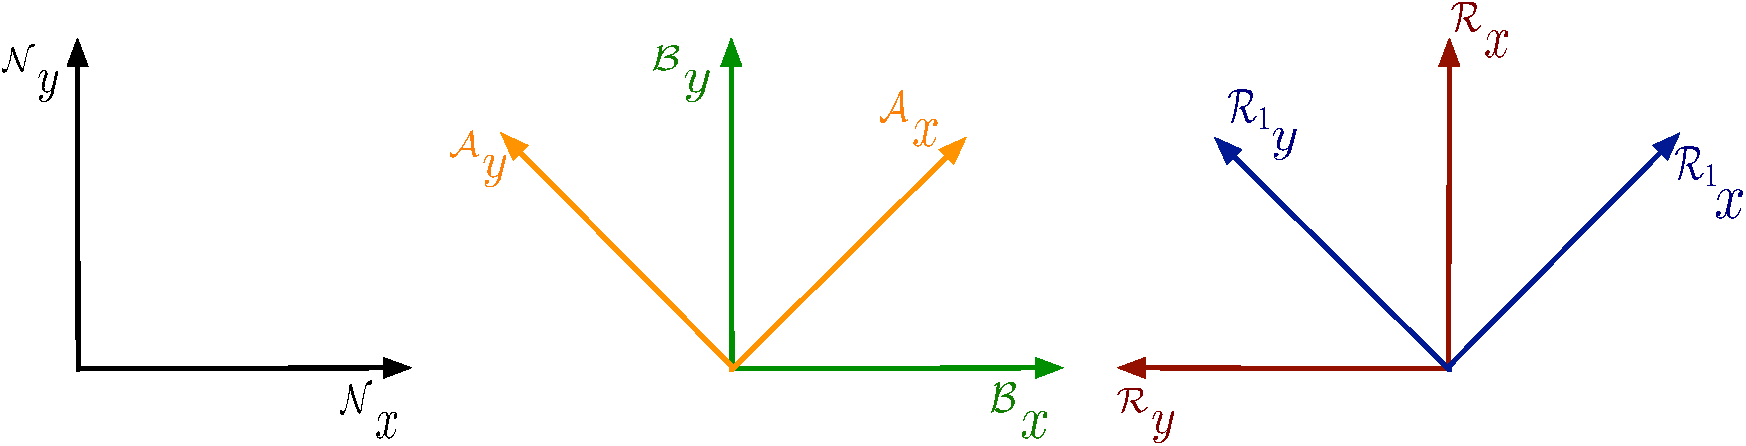
\includegraphics[scale=0.5]{Figures/Coordinate_systems.pdf}
	}
	\caption{Aligning coordinate systems example}
	\label{fig:coordinate_systems}
\end{figure}